
\chapter[]{Modularisation des systèmes distribués}% TODO: maybe rename.
%%% - Programme/Processus
%%% - Exécutable

Les programmes modernes ont une structure \textit{modulaire},
c'est-à-dire que leur code se décompose logiquement en différentes
parties relativement indépendantes, les \textit{modules}.  Cette
structure a de nombreux avantages, entre autres sur le plan du
développement et de la maintenance.  La structure d'un programme en
vue de son \textit{déploiement} -- c'est-à-dire comment son code
exécutable est stocké sur disque, chargé en mémoire, etc. -- peut prendre
plusieurs formes.

Un programme sous forme \textit{monolithique} contient dans son code exécutable
toutes les instructions exécutées par l'ordinateur.  Cette forme était la norme
dans les premiers systèmes informatiques, et l'est toujours pour les systèmes
embarqués qui n'ont pas de système d'exploitation indépendant.  Lorsqu'un
système d'exploitation est disponible sur l'ordinateur on peut le considérer
comme étant un module puisqu'il offre des services précis avec une interface
standardisée.  Dans ce cas, un programme peut prendre la forme d'un seul
fichier de code qui, à son exécution, communiquera avec le système
d'exploitation pour accéder à ses services.  Ce genre de fichier exécutable est
obtenu par une \textit{édition de liens statique} qui combine en un seul
fichier tous les modules (à l'exception du système d'exploitation).  Par
rapport à la forme monolithique, cette organisation simplifie le développement
car le programmeur n'a pas à se soucier du développement des services de base
comme l'accès aux fichiers, la gestion des processus et de la mémoire, etc.  Le
programme peut être distribué à d'autres ordinateurs ayant le même système
d'exploitation simplement en y transférant le fichier exécutable.

L'édition de lien statique a un certain nombre de défauts. La version des
modules utilisé au moment de l'édition de liens est figée au sein du
programme, ce qui empêche la mise à jour individuelle des modules. Il faut
recompiler tous les modules qui ont subi une mise à jour et refaire l'édition de liens du
programme principal. Le coût en temps et l'effort pour un changement minime
est important.  Le chapitre \ref{ch:loading-model} va détailler plus en profondeur
ces problèmes.

% Le même module est chargé plus d'une fois.
L'édition de liens peut se faire paresseusement par le système d'exploitation à
l'exécution du programme, ce qu'on appelle l'\textit{édition de liens dynamique}.  Cela
permet de garder la structure modulaire au \textit{déploiement}.
Chaque module est une composante séparée du programme principal.  Ces modules
sont lus du disque et chargés en mémoire durant l'exécution du programme.  Ce
chargement est effectué par \textit{éditeur de liens dynamique} qui s'occupe de
lié les fonctionnalités des modules au programme principal. Le chapitre % chapter or section
\ref{ch:module_systems} explique plus en profondeur le fonctionnement de éditeur de liens
dynamique. L'avantage principal du chargement dynamique de module est la mise à jour
individuelle d'un module sans avoir a lié le programme principale; dans le
modèle statique le programme principal doit être lié à nouveau avec les modules.
Les modules chargés dynamiquement par le système d'exploitation peuvent être partagé entre différent
programme. Ce type de module porte le nom de \textit{bibliothèque partagée} ils sont décrit dans
le chapitre \ref{ch:module_systems}.

% % Migration de code dans un système distribué.
% - Transmission de tâche entre des machines d'un système distribué.
%   - Un module absent sur la machine distante nécessaire à l'exécution
%   de la tâche transmise.
%     - Télécharger le module d'un serveur dédié.
%     - Revient au chargement dynamique de ce module.
\section{Systèmes distribués}


Un programme distribué est séparé sur plusieurs systèmes. Dans un système
distribué, il est possible de transmettre des tâches entre les différents
systèmes. C'est ce qu'on appelle, \textit{migration de tâche}.  Un exemple de
migration de tâche est l'invocation de \texttt{ssh} qui permet d'exécuter un
processus sur un système distant. Le problème de cette approche est que le
programme doit exister sur la machine distante et que chaque invocation passe
par une authentification. Des mécanismes de migration de code ont été
implémentés dans différents langages comme Erlang~\cite{M_mobileintelligent},
Java~\cite{And98transparentmigration}, Scheme~\cite{Sumii00animplementation},
Javascript~\cite{DEV2017transparentmigration}, \dots.  La plupart des méthodes
de migration de code requièrent que l'ensemble des procédures sont
présentes sur le système distant.

Le système Java~\cite{And98transparentmigration} capture l'état du programme courant
qui consiste aux valeurs et aux types de toutes les variables de chaque objet. L'autre
information est la pile des appels de méthode avec les valeurs de toutes les variables.
Ces informations sont transmis et utilisés pour reconstruire l'état du programme.
L'ensemble des méthodes sur le nœud de départ est présent sur le nœud d'arrivé.
Le système Erlang~\cite{M_mobileintelligent} requière aussi que le code soit disponible
sur le nœud destination.

Le système de migration en Javascript utilise des dépôts de code pour conserver
le code. Il est basé sur le fait que le code des agents sont connus par des
nœuds spécialisés. Puisque le code des agents est connu, il suffit de
transmettre l'état de l'agent. Ce modèle Javascript ressemble à celui
implémenté dans Gambit lors de la transmission de procedure compilé.

La migration de de code ne devrait pas être limité par le code sur le nœud
distant. Le système de module offre la possibilité de migrer un agent sur un
nœud qui ne connait pas le code de l'agent. Un exemple concret de migration
de code est présenté dans le chapitre \ref{ch:task_migration}. Le problème
est la migration de code sur un nœud qui ne connait pas le code de l'agent qui
est migrer.


\section{Modules versionnés}
%
Un programme est généralement composé de plusieurs modules. Chaque module est
associé à une seule version. La façon qu'un système voit les versions d'un
module diffère entre les langages. Il est possible de voir chaque version d'un
module comme un module différent, c'est ce qui est utilisé dans Go. Dans les
système comme Python et Java les modules sont vus par le programme par seulement
un nom qui n'inclut pas la version.

Dans les système qui considère chaque version d'un module comme un module différent,
il existe des programmes qui chargent plusieurs versions d'un module. Cela peut amener
certains problèmes de conflit entre les versions du module. Ces conflits peuvent être
observer dans les langages interprété comme Javascript ou dans les langages compilé
comme C/C++. Les conflits peuvent être dans les noms des fonctions du module ou
dans des variables globales partagés entre plusieurs versions du module. Le chapitre
\ref{ch:module_systems} traite des différent cas de conflit avec des exemple
dans plusieurs langages programmations.

% XXX: Agent TCL

% \section{Linkage statique}
% Cette forme d'édition de lien permet la création de binaire qui indépendant
% qui facilite le déploiement.

%\section{Linkage dynamique}

%--------------------------END---------------------------

% TODO: move to chapter task_migration
% Un programme sur une des machine du système distribué qui se fait transmettre
% une tâche peut devoir exécuter une fonctionnalité d'un module absent
% localement. Cela nécessite un téléchargement du module contenant la
% fonctionnalité demandé d'un serveur dédié. Une fois le module installé, il faut
% le charger dynamiquement.

% ==> motiver (quels problèmes ça cause le link statique) et expliquer le chargement dynamique, système distribué, etc
% TODO lien => liens


%Problème du link statique\\
% - Gèle les versions des modules au sein du programme. \\
%    -> Comment la maintenance d'un programme lié statiquement? \\
%    - Le temps de compilation. (Coût d'un changement est important) \\
% - La taille du programme peut être plus importante.
% - Le même module est chargé plusieurs fois en mémoire.



% Dans les systèmes comme DOS, les programmes ou modules devaient contenir toutes les
% informations nécessaire pour s'exécuter. De tels programmes sont dit lié
% statiquement dans le sens qu'il ne dépende que de l'architecture sur laquelle il
% a été construit. La construction des modules requière deux étapes. La compilation
% de fichier source en fichier objet contenant le nom et le code des fonction.
% L'édition des liens qui réunit un plusieurs fichiers objets en un module.
% Dans le cas d'un seul fichier l'édition des liens ne fait que transformer le fichier
% objet en fichier exécutable.

% \begin{figure}[ht]
%   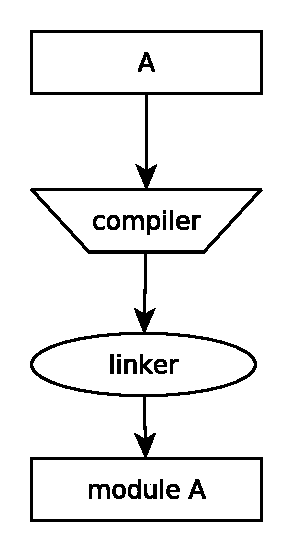
\includegraphics[width=0.20\linewidth]{figures/basic_module_compilation.pdf}
%   \caption{Construction du module A à partir des sources.}
% \end{figure}

%La création d'exécutable inclut deux étapes importantes, la compilation et
%l'édition des liens. La première étape consiste à prendre un fichier de code
%source et de le traduire en fichier objet, que l'on retrouve souvent avec
%l'extension \verb|.o| ou \verb|.obj|, qui contient la représentation des
%procédures compréhensible par le processeur. Ces fichiers objets ne sont pas
%encore exécutable pour autant, il faut tout d'abord effectuer la seconde étape,
%qui va les regrouper en un exécutable. Le programme qui s'occupe de l'édition
%des liens est le \textit{linker}, la version GNU se nomme \verb|ld|.  Voici
%l'exemple de la création d'un exécutable composé des fichiers sources C
%\verb|main.c| et \verb|foo.c|:
%
%\begin{figure}[ht]
%    \begin{minipage}[t]{0.5\textwidth}
%\begin{verbatim}
%# Compilation
%gcc -c main.c -o main.o
%gcc -c foo.c -o foo.o
%# Édition de liens
%ld -o main.exe main.o foo.o
%\end{verbatim}
%    \end{minipage}
%
%    \caption{Exemple de création d'un exécutable}
%\end{figure}



%Cela implique que ils possible de retrouvé une dépendance en diamant tel que représenter
%dans la figure-\ref{fig:dep1} qui peut causer un problème. % Détailler
%\begin{figure}[ht] %% Pas juste valide pour scheme.
%  \begin{center}
%    %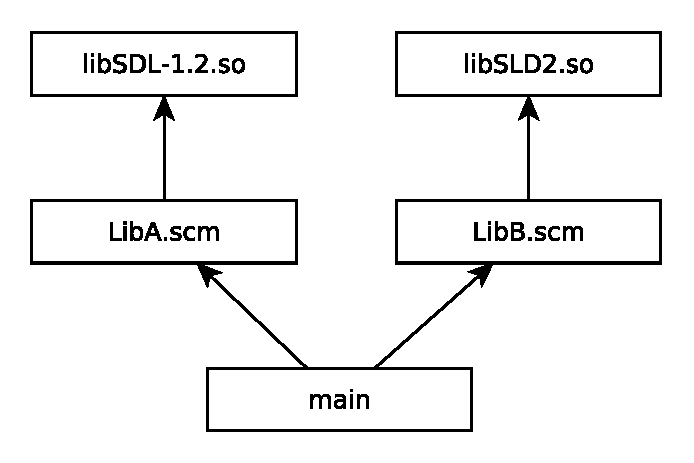
\includegraphics[width=4cm]{figures/SchemeLibrary}
%    \caption{Dépendence en diamant}
%    \label{fig:dep1}
%  \end{center}
%\end{figure}

%% NOTE: Soit P un processus, execution(A, P=[A,B]) == execution(A, P=[A]).
%Soit un processus \textbf{P} qui réfère aux bibliothèques \textbf{A} et \textbf{B}.
%Une bibliothèque peut masquer les symboles d'une autre bibliothèque chargé dans le même processus.
%La bibliothèque \textbf{A} coexiste avec la bibliothèque \textbf{B} si la \textbf{A}
%ne masque pas des symboles ne \textbf{B} qui amène un comportement non défini.


% Historiquement, il y avait un problème avec la coexistence entre deux dll sous Window. TODO: devellopper

% - Système distribué (Actor), non limité par la diversité des bibliothèque.


% TODO:
%La coexistance entre plusieurs versions d'une même bibliothèque
%===========================================================
%
% - Définition d'une bibliothèque
%   - Nom symboles:
%     - Fonction
%     - Variables global
%     - Structure de donnée
%     - Macro (Compilation)
%
%- Définition par coexistence de plusieurs bibliothèque.
%- Pourquoi est-ce utile?
%- Conditions nécessaire pour la coexistence entre plusieurs versions d'une même bibliothèque soit possible.
%  - Data race.
%  - État partagé.
%- Système d'exploitation (DOS)


